\documentclass{article}
    \title{\textbf{2b. VLIV TVARU KŘIVKY NA ÚDAJ MĚŘICÍHO PŘÍSTROJE}}
    \author{Tomáš Kysela}
    \date{14/3/2022}

    \addtolength{\topmargin}{-3cm}
    \addtolength{\textheight}{3cm}

\usepackage[czech]{babel}
\usepackage{float}
\usepackage{graphicx}
\usepackage{circuitikz}
\usepackage{amsmath}
\usepackage{subcaption}
\usepackage{pgfplots}
\usepackage{siunitx}
\sisetup{detect-all}

\makeatletter
\providecommand\add@text{}
\newcommand\tagaddtext[1]{%
    \gdef\add@text{#1\gdef\add@text{}}}%
\renewcommand\tagform@[1]{%
    \maketag@@@{\llap{\add@text\quad}(\ignorespaces#1\unskip\@@italiccorr)}%
}
\makeatother


\begin{document}

\maketitle

\section{Úkol měření}
\begin{enumerate}
	\item Změřte napětí na zátěži, jejíž výkon je regulován obvodem s triakem pro úhel sepnutí $\alpha$ přibližně 0\si{\degree}, 45\si{\degree} a 90\si{\degree} předloženými číslicovými multimetry $V_1$ až $V_4$.
	\item Průběh napětí sledujte na osciloskopu (osciloskop připojte na výstup odporového děliče).
	\item Určete, které z multimetrů měří správně efektivní hodnotu, a určete relativní chybu metody měření efektivní hodnoty u ostatních.
	\item Z údaje multimetrů, které to umožňují, určete aritmetickou střední hodnotu měřeného průběhu.
	\item Pro úhel sepnutí $\alpha = 90\si{\degree}$ určete aritmetickou střední hodnotu a efektivní hodnotu napětí rovněž výpočtem z definic. Vypočtené hodnoty srovnejte s naměřenými a v případě jejich rozdílu analyzujte možné příčiny.
\end{enumerate}
\section{Schéma zapojení}
\begin{figure}[h]
	\centering
	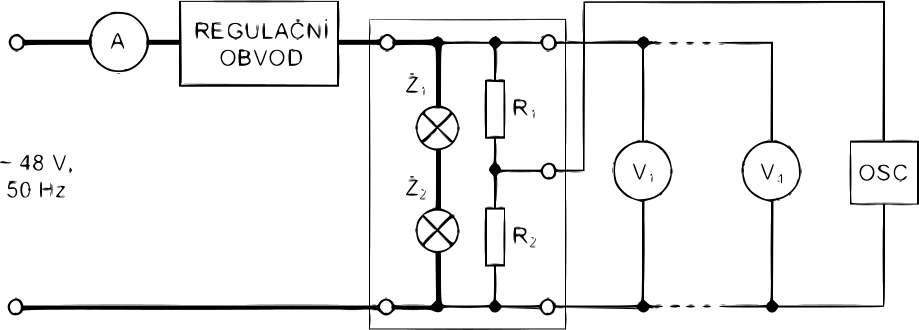
\includegraphics[width=0.7\linewidth]{scheme1}
	\caption{Zapojení měřícího obvodu}
	\label{fig:scheme1}
\end{figure}
\begin{figure}[H]
	\centering
	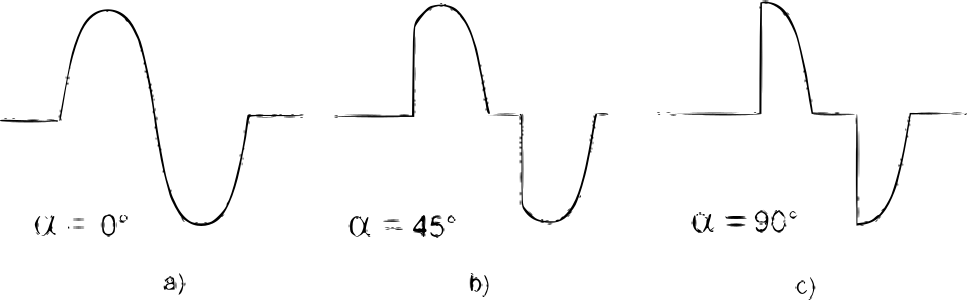
\includegraphics[width=0.6\linewidth]{scheme2}
	\caption{Průběhy měření napětí}
	\label{fig:scheme2}
\end{figure}

\section{Soupis použitých přístrojů}
\begin{tabular}{ll}
	$A$ & ampérmetr elektromagnetický \\
	$Z$ & přípravek se dvěma žárovkami $Z_1$, $Z_2$ a odporovým děličem $R_1$, $R_2$ \\
	$V_1$ & číslicový multimetr HP 34401A, rozsah 1 V a 10 V \\
	$V_2$ & číslicový multimetr Summit 45, rozsah 4 V a 40 V \\
	$V_3$ & číslicový multimetr MY-64 (Mastech), rozsah 2 V a 20 V \\
	$V_4$ & nízkofrekvenční elektronický voltmetr Troneer, rozsah 1 V a 10 V \\
	Regulační obvod & přípravek pro regulaci průběhu proudu
\end{tabular}
\section{Teoretický základ}
Voltmetry měřící střídavé napětí používají pro převod střídavého napětí na stejnosměrné
převodníky střední nebo efektivní hodnoty.
Levnější přístroje využívají převodníky střední hodnoty pomocí operačního usměrňovače.
Přístroje očekávají sinusový průběh, změří střední aritmetickou hodnotu podle vztahu
\begin{equation}
	U_{sar}=\frac{1}{T}\int_{0}^{T}|u(t)|dt=\frac{2}{T}\int_{0}^{T/2}u(t)dt
\end{equation}
,kterou přenásobí koeficientem 1,11, čímž získají efektivní hodnotu
\begin{equation}
	U_{ef} = 1.11 \cdot U_{sar}
\end{equation}
Pokud však měřený signál nemá sinusový průběh, koeficient převodu je jiný než 1,11 a přístroje ukazují nesprávnou hodnotu.
Kvalitnější přístroje používají převodníky efektivní hodnoty, což je často označováno jako
\textit{True RMS}. Měří tedy efektivní hodnotu signálu podle definičního vztahu
\begin{equation}
	U_{ef} = \sqrt{\frac{1}{T}\int_{0}^{T}u^2(t)dt}=\sqrt{\frac{2}{T}\int_{0}^{T/2}u^2(t)dt}
\end{equation}
bez ohledu na to, zda má signál sinusový průběh či nikoli.

Vztah pro sinusový průběh (4), jeho periodu (5) a amplitudu (6).
\begin{equation}
	u(t)=U_m\sin(\omega t)
\end{equation}
\begin{equation}
	T=\frac{2 \pi}{\omega}
\end{equation}
\begin{equation}
	U_m=\sqrt{2}\cdot U_{ef}
\end{equation}
Dosazením do vztahů (1) a (3) s úhlem sepnutí $\alpha$ a dobou sepnutí $t_\alpha = \frac{T\cdot\alpha}{2\pi}=\frac{\alpha}{\omega}$ získáme vzorce pro střední (7) a efektivní (8) hodnotu při posunutí $\alpha$.
\begin{equation}
	U{sar,\alpha}=\frac{2}{T}\int_{\alpha/\omega}^{T/2}U_m\sin(\omega t)dt=\frac{U_m}{\pi}[\cos(\alpha)-\cos(\pi)]
\end{equation}
\begin{equation}
	U_{ef,\alpha}=\sqrt{\frac{2}{T}\int_{\alpha/\omega}^{T/2}U_m\sin^2(\omega t)dt} = \frac{U_m}{\sqrt{2\pi}}\sqrt{\pi-\alpha+\frac{\sin(2\alpha)}{2}}
\end{equation}
\end{document}
